\documentclass[10pt,a4paper]{article}
\usepackage{ifpdf}
\usepackage[utf8]{inputenc}
\usepackage[T1]{fontenc}
\usepackage[francais]{babel}
\usepackage{lmodern}
\usepackage{graphicx}
\usepackage{amsmath}
\usepackage{amsfonts}
\usepackage{amssymb}
\usepackage{enumitem}
\usepackage[margin=1.5cm]{geometry}
\usepackage{hyperref}
\usepackage{url}

\title{Projet de Physique Numérique : Mesure de distances par stéréoscopie}
\author{Lucas Verney}
\date{2012/2013}
\ifpdf
\pdfinfo {
	/Author (Lucas Verney)
	/Title (Projet de Physique Numérique : Mesure de distances par stéréoscopie)
}
\fi
\begin{document}
	\maketitle
	
	\section{Objectif}
		Le but de ce projet était de déterminer des distances séparant un observateur d'un objet à partir de deux photos de cet objet prises en déplaçant horizontalement l'appareil entre les prises de vue. En utilisant la stéréoscopie, on peut en effet déterminer la distance nous séparant de l'objet, tout comme notre cerveau est capable d'estimer les distances nous séparant des objets à partir des ``images'' captées par nos yeux.
		
		\bigskip
		
		\underline{\emph{Exemple :}}
		\medskip
		
		\begin{center}
			\begin{tabular}{cc}
				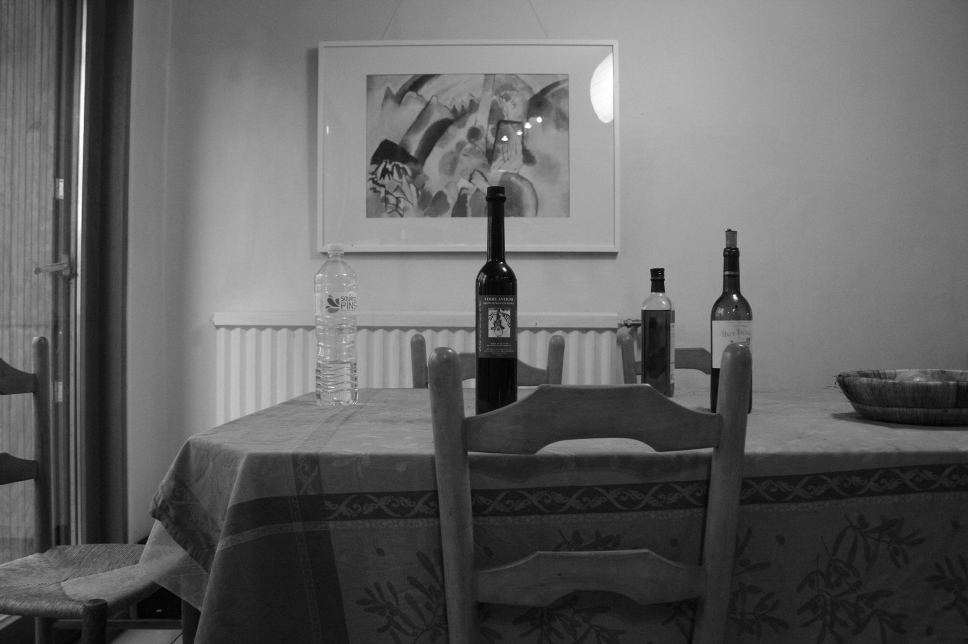
\includegraphics[scale=0.25]{IMG_0114s.JPG} & 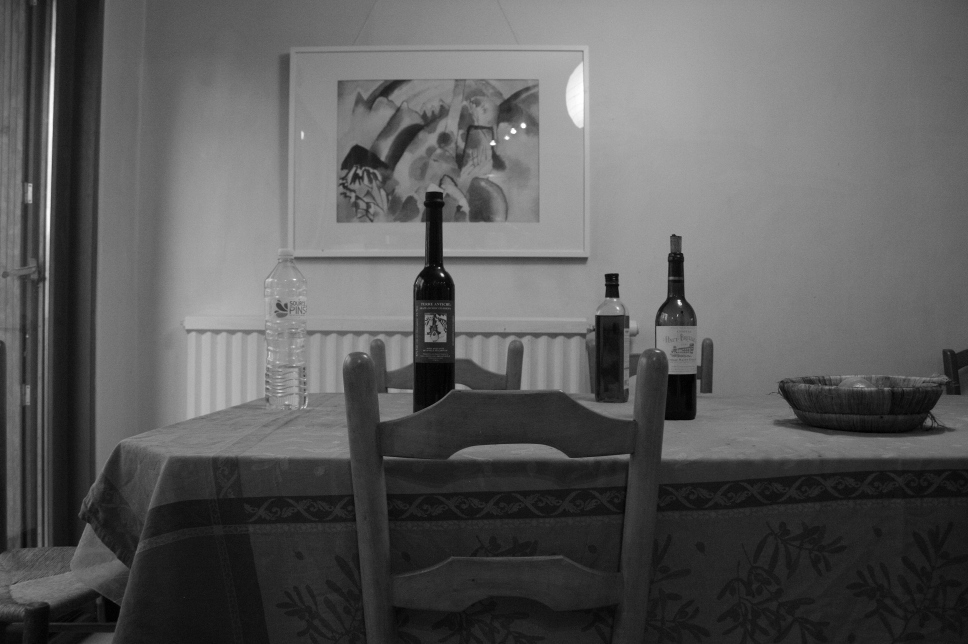
\includegraphics[scale=0.25]{IMG_0115s.JPG} \\
				\emph{Image de gauche} & \emph{Image de droite} \\
			\end{tabular}
		\end{center}
		
	\section{Méthode choisie}
		Il faut, dans un premier temps, déterminer le déplacement en pixels de l'objet entre les deux images. Dans un deuxième temps, il faut traduire ce déplacement en distance réelle nous séparant de l'objet.
		
		\subsection{Distance euclidienne dans l'espace RGB}
			Pour déterminer le déplacement en pixels, on considère une grille de $n\times n$ pixels, qu'on superpose à notre image de gauche (par défaut, $n = 50$ dans le programme). Pour chaque carrés de $n\times n$ pixels, on cherche le carré qui lui correspond le plus dans l'image de droite. Pour ce faire, on va parcourir chaque pixel de l'image de droite et comparer le carré de l'image de gauche et le carré dont le coin supérieur gauche est le pixel courant dans l'image de droite. 
		
			Les images étant chargées en couleur (RGB), on est dans un espace à trois dimensions (R, G et B) dont les coordonnées des pixels sont entre $0$ et $255$ (profondeur de couleur de 8 bits). On peut donc estimer la ``distance'' séparant les deux carrés par la moyenne sur le carré des distances pixel à pixel où la distance pixel à pixel est la distance euclidienne standard ($=\sqrt{(R_2 - R_1)^2 + (G_2 - G_1)^2 + (B_2 - B_1)^2}$).
		
		\subsection{Cross-correlation \emph{via} FFT}
			Une autre possibilité est d'utiliser la cross-correlation (ou la phase correlation) afin de déterminer la position de notre objet.
			
			On commence par charger les images en niveaux de gris et on récupère le carré qu'on considère dans une nouvelle image, de la même taille que l'image de droite. On complète cette image par du noir (des 0) qui n'interviendront donc pas dans la transformation de Fourier.
			
			On effectue ensuite les transformations de fourier de chaque image et on multiplie le spectre de l'image de droite par le conjugué du spectre du carré dont on cherche la position. On normalise ensuite la transformation de Fourier (en divisant chaque la valeur de chaque point par son module) et on repasse en espace réel (\emph{via} une transformation de Fourier inverse.
			
			On cherche ensuite la valeur de la plus grande amplitude sur cette image, qui correspond à la position du carré qu'on cherche.
		
		\bigskip
		
		Une fois cette distance déterminée, on peut en déduire la distance nous séparant de l'objet en utilisant les formules explicitées dans \cite{article}. Connaissant les caractéristiques de l'appareil, il est facile de traduire le déplacement en pixels précédent en distance réelle.
	
	\section{Résultats}
		Le programme obtenu a été testée sur le jeu d'images suivant (les tests ont été effectués en considérant le coin inférieur gauche du carré noir) :
		
		\begin{center}
			\begin{tabular}{cc}
				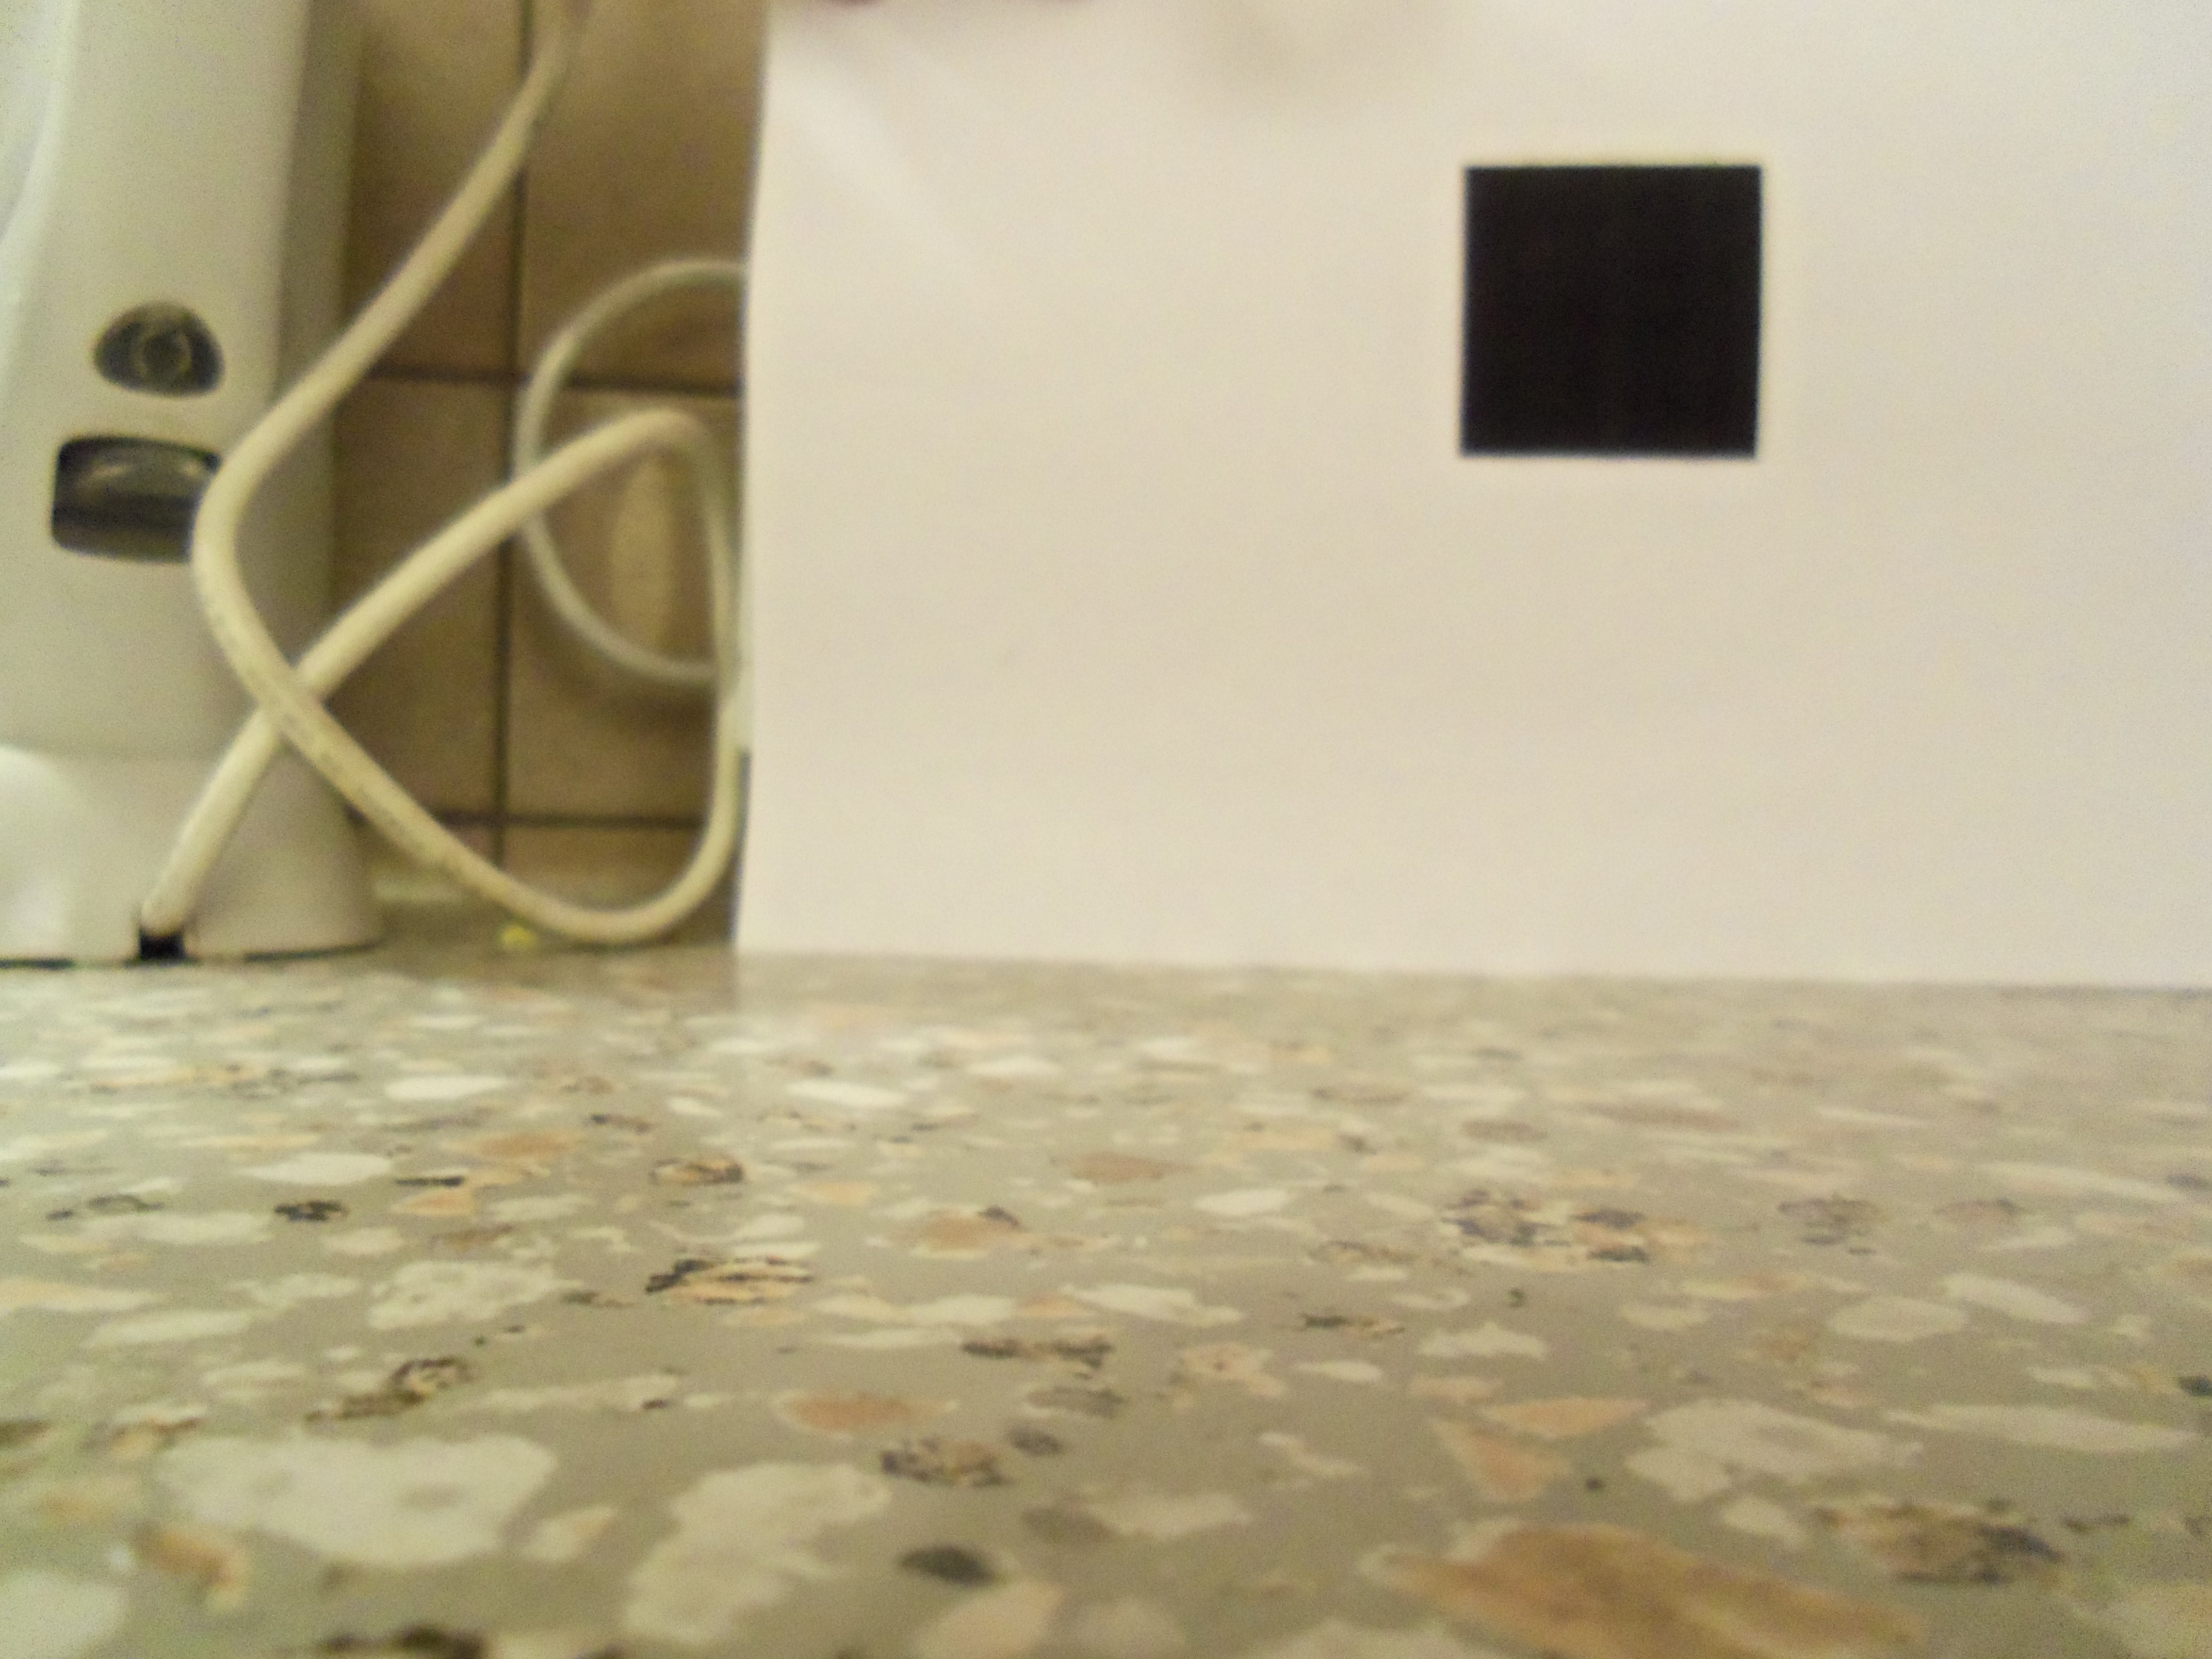
\includegraphics[scale=0.05]{Left.JPG} & 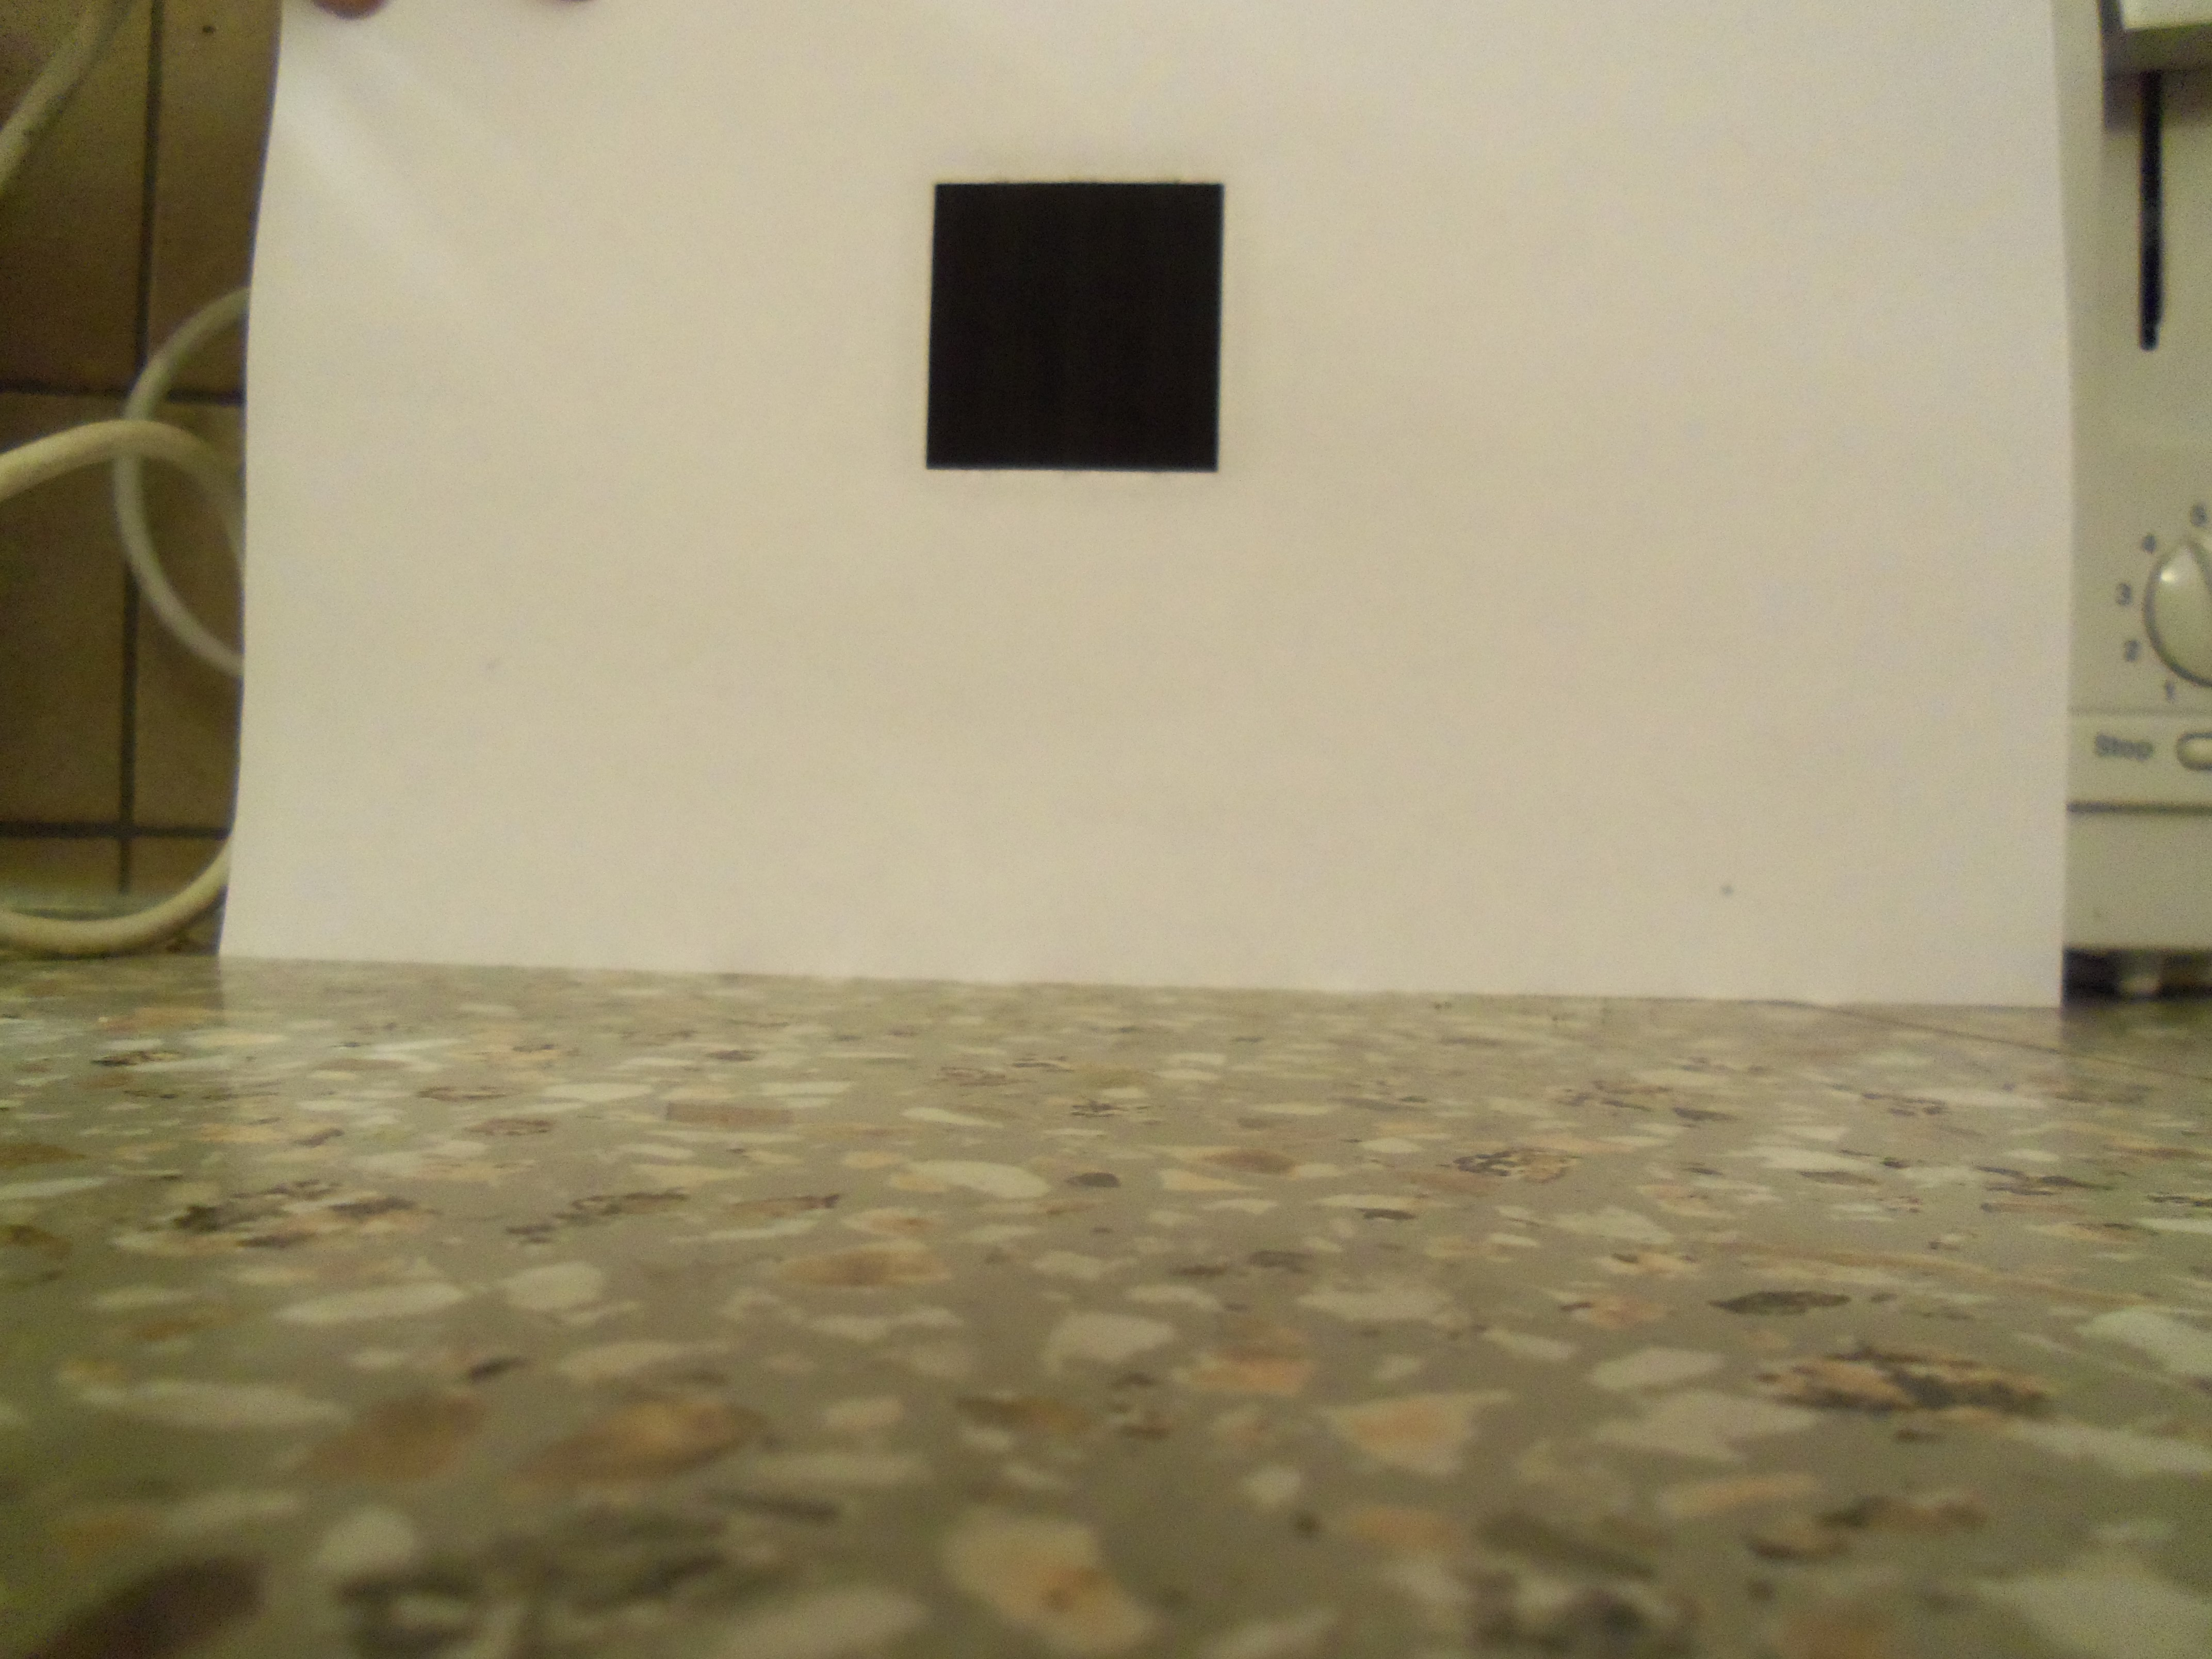
\includegraphics[scale=0.05]{Right.JPG} \\
				\emph{Image de gauche} & \emph{Image de droite} \\
			\end{tabular}
		\end{center}
		
		Le programme décrit précédemment permet de déterminer très précisément le déplacement du coin inférieur gauche et on ne peut obtenir une meilleure précision manuellement. Ce résultat a été obtenu en une vingtaine de secondes en utilisant les $4$ c{\oe}urs du processeur, ce qui est relativement long. En effet, pour parcourir toute l'image avec la méthode précédente et des carrés de $50$ pixels de large, il faudrait environ $30h$.
		
		Après conversion du déplacement en pixels en distance réelle, on trouve une distance réelle de $15cm$ contre $35cm$ en réalité (en utilisant des caractéristiques ``moyennes'' pour l'appareil photo). Cependant, le déplacement étant convenablement détecté, cet écart provient d'une méconnaissance des caractéristiques précises de l'appareil photo utilisé (notamment sa distance focale).
		
		En conclusion, cette technique nous permet de déterminer des distances très précisément mais est très coûteuse en ressources et il est difficilement envisageable de couvrir une photo entière avec cette méthode.
		
		La technique utilisant la transformée de fourier rapide est nettement plus rapide (une vingtaine de secondes par image) et donne des résultats légèrement moins précis mais largement comparables.
		
		\medskip
		\emph{Remarque :} Il faut également noter qu'on ne détermine pas la distance nous séparant d'un objet (ou d'un point) précis mais une moyenne de cette distance sur un carré de $n$ pixels de large. Il faut donc choisir la taille de ce carré petite devant l'échelle caractéristique de variation des distances (liée à la taille transversale des objets).
		
		\emph{Remarque :} On peut également utiliser un algorithme de détection de contours (type filtre de Sobel qui calcule le ``gradient'' de l'image) pour travailler sur une image en niveau de gris et déterminer les distances nous séparant des contours des objets, ceci afin d'obtenir une meilleure précision sur des images chargées.
	
	\section{Optimisations possibles}
		Comme on l'a vu précédemment, la méthode employée est très coûteuse en ressources. On peut envisager diverses optimisations :
		\begin{itemize}
			\item On peut envisager d'appliquer un filtre de détection de contours (type filtre de Sobel) avant de travailler sur l'image. On peut alors se restreindre aux zones d'intérêt, c'est-à-dire aux contours représentés par des pixels blancs.
			\item Pour accélérer le calcul des distances, on peut envisager de paralléliser au maximum les opérations. Dans le code présenté, on utilise jusqu'à $4$ c{\oe}urs du processeur mais l'utilisation de la puce graphique pourrait accélérer le calcul, celle-ci travaillant naturellement avec des calculs parallèles.
			\item Jusqu'ici, on n'a envisagé qu'un déplacement horizontal (ou vertical en travaillant sur une image retournée). On pourrait envisager le cas d'un déplacement quelconque dans l'espace (translation) en adaptant les formules.
		\end{itemize}
	
	\nocite{article2}
	\nocite{templateMatching}
	\nocite{phaseCorrelation}
	
	\bibliographystyle{plain-fr}
	\bibliography{biblio}
\end{document}